\section{Appendix: \LaTeX\ Tips}

If you want to add a mathematical equations, put the large equation in this way:
\begin{equation}
result = \sum_{i=0}^N \mathcal{F}(e_i, t_i, p_i),
\end{equation}
where $e_i$, $t_i$, $p_i$ stands for the effort, time, and practice for the time stamp $t$, respectively. If you want to add equations in the text, use \$your\_equation\$. The inline equation shall be look like $\sum_i \alpha$. If you are interested in available characters and fonts in Latex, please refer to the nice materials from OverLeaf~\footnote{\url{https://www.overleaf.com/learn/latex/List_of_Greek_letters_and_math_symbols}}.

To put a picture, consider the following examples.
\begin{figure}
    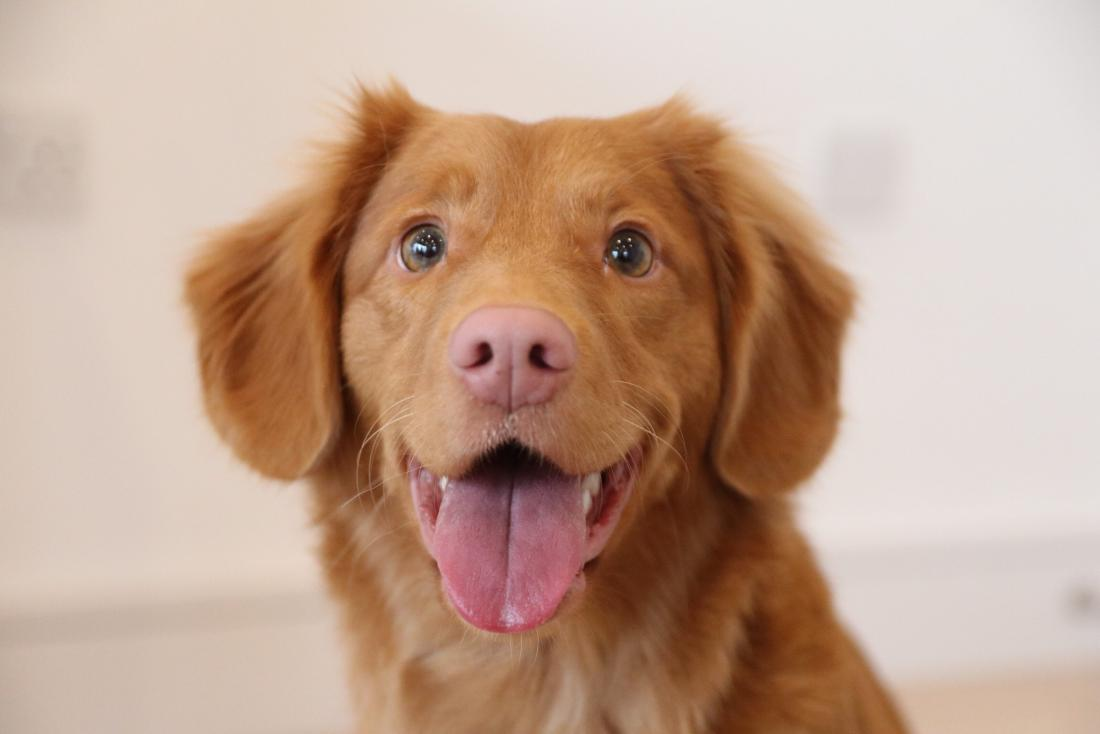
\includegraphics[width=\linewidth]{dog.jpg}
    \caption{You can put a picture and caption in this way. Image taken from Medical News Today.}
\label{fig:dog}
\end{figure}
You can refer the picture in this way. "Fig.~\ref{fig:dog} shows a cute dog. According to Dr. Park, having a pet makes you healthy."
Tou can use the following example to put a table. You can refer "Table.~\ref{table:example} shows a nice results on the xx experiments.."
\begin{table}
\begin{center}
    \begin{tabular}{|l|c|}
    \hline
    Method & Frobnability \\
    \hline\hline
    Theirs & Frumpy \\
    Yours & Frobbly \\
    Ours & Makes one's heart Frob\\
    \hline
    \end{tabular}
\end{center}
\caption{Results.   Ours is better.}
\label{table:example}
\end{table}

To put a comprehensive picture, you can consider any GUI-based image editing software such as photoshop, illustrator, or even PowerPoint. You can export the figure as pdf, jpeg, png. If your picture has some texts, definitely consider using pdf format. Texts in a jpeg and png image will be rasterized, so it will end up losing the beautiful vector graphics.
